% Professional text-free logo from a coding-theory perspective
% Standalone TikZ source for presentation/tikzs/logo.pdf
\documentclass[tikz, border=14pt]{standalone}

\usepackage{xcolor}

\usetikzlibrary{
	arrows.meta,
	calc,
	decorations.markings,
	shapes.geometric
}

\definecolor{inkC}{HTML}{101A24}
\definecolor{paperC}{HTML}{F8FBFC}
\definecolor{gridC}{HTML}{DDE8EA}
\definecolor{codeC}{HTML}{008C8C}
\definecolor{fieldC}{HTML}{3155A4}
\definecolor{cryptoC}{HTML}{B87511}
\definecolor{errC}{HTML}{D33F49}

\begin{document}
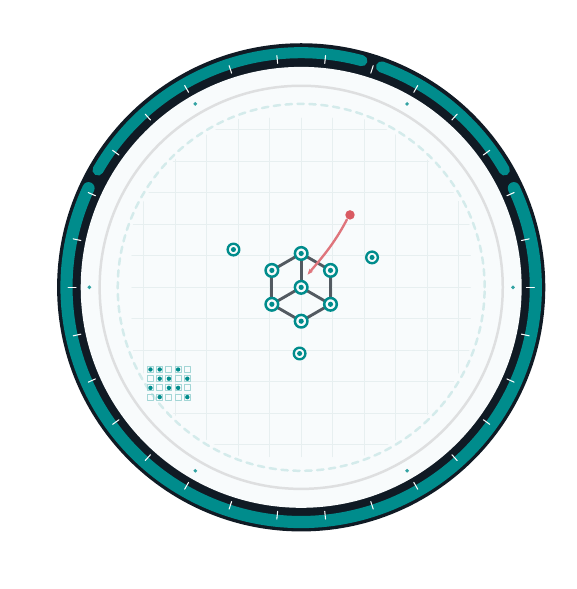
\begin{tikzpicture}[
	x=1cm,
	y=1cm,
	line cap=round,
	line join=round
	]
	
	% Badge geometry
	\def\Rbadge{3.10}
	\def\Rinner{2.80}
	\coordinate (C) at (0,0);
	
	% Outer badge: coding theory gets the dominant teal arc.
	\fill[inkC] (C) circle (\Rbadge);
	\draw[codeC, line width=4.4pt] (155:2.98) arc[start angle=155, end angle=385, radius=2.98];
	\draw[codeC, line width=4.0pt] (75:2.98) arc[start angle=75, end angle=150, radius=2.98];
	\draw[codeC, line width=4.0pt] (30:2.98) arc[start angle=30, end angle=70, radius=2.98];
	\fill[paperC] (C) circle (\Rinner);
	\draw[inkC!14, line width=0.9pt] (C) circle (2.56);
	\draw[codeC!17, line width=0.9pt, dash pattern=on 2.3pt off 2.0pt] (C) circle (2.33);
	
	% Register marks around the coding rim.
	\foreach \ang in {0,12,...,348}{
		\draw[paperC!56, line width=0.38pt] (\ang:2.86) -- (\ang:2.96);
	}
	\foreach \ang in {0,60,...,300}{
		\fill[codeC!80] (\ang:2.69) circle (0.025);
	}
	
	% Ambient finite-field coordinate grid, kept faint.
	\begin{scope}
		\clip (C) circle (2.28);
		\foreach \x in {-2.0,-1.6,...,2.0}{
			\draw[gridC!70, line width=0.35pt] (\x,-2.15) -- (\x,2.15);
		}
		\foreach \y in {-2.0,-1.6,...,2.0}{
			\draw[gridC!70, line width=0.35pt] (-2.15,\y) -- (2.15,\y);
		}
	\end{scope}
	
	% Code space: three Hamming balls and Voronoi-like boundaries.
%	\foreach \x/\y/\r/\op in {-0.86/0.48/0.82/16, 0.90/0.38/0.74/14, -0.02/-0.84/0.78/15}{
%		\fill[codeC!\op] (\x,\y) circle (\r);
%		\draw[codeC!34, line width=0.65pt] (\x,\y) circle (\r);
%		\draw[codeC!22, line width=0.45pt, dash pattern=on 2pt off 1.8pt] (\x,\y) circle ({0.66*\r});
%	}
%	\draw[inkC!16, line width=1.2pt] (-0.18,1.14) -- (0.24,-1.64);
%	\draw[inkC!16, line width=1.2pt] (-1.55,-0.18) -- (1.62,0.95);
%	\draw[inkC!16, line width=1.2pt] (-1.02,1.17) -- (1.20,-1.23);
	
	% Central codeword: seven coordinates in a compact block-code constellation.
	\coordinate (q0) at (0,0);
	\foreach \name/\ang in {q1/90,q2/30,q3/-30,q4/-90,q5/-150,q6/150}{
		\coordinate (\name) at (\ang:0.43);
	}
	\foreach \a/\b in {q1/q2,q2/q3,q3/q4,q4/q5,q5/q6,q6/q1,q0/q1,q0/q3,q0/q5}{
		\draw[inkC!72, line width=1.05pt] (\a) -- (\b);
	}
	\foreach \p in {q0,q1,q2,q3,q4,q5,q6}{
		\fill[paperC] (\p) circle (0.080);
		\draw[codeC, line width=0.90pt] (\p) circle (0.080);
		\fill[codeC] (\p) circle (0.033);
	}
%	\node[
%	regular polygon,
%	regular polygon sides=6,
%	rotate=30,
%	minimum size=1.23cm,
%	inner sep=0pt,
%	fill=codeC,
%	fill opacity=0.96,
%	draw=paperC,
%	line width=0.9pt
%	] at (C) {};
%	\foreach \p in {(0,0.24),(0.21,-0.12),(-0.21,-0.12)}{
%		\fill[paperC] \p circle (0.052);
%	}
%	\draw[paperC!78, line width=0.72pt] (0,0.24) -- (0.21,-0.12) -- (-0.21,-0.12) -- cycle;
%	\fill[errC] (0,0) circle (0.032);
%	\draw[errC, line width=0.82pt] (C) circle (0.63);
	
	% Received word and nearest-neighbor decoding arrow.
	\fill[errC!86] (0.62,0.92) circle (0.060);
	\draw[errC!72, line width=0.85pt, -{Stealth[length=2.2pt]}]
	(0.58,0.86) .. controls (0.42,0.55) and (0.24,0.35) .. (0.08,0.16);
	\foreach \p in {(-0.86,0.48),(0.90,0.38),(-0.02,-0.84)}{
		\fill[paperC] \p circle (0.074);
		\draw[codeC, line width=0.85pt] \p circle (0.074);
		\fill[codeC] \p circle (0.032);
	}
	
	% Left satellite: generator-matrix structure without characters.
	\begin{scope}[shift={(-1.68,-1.16)}, scale=0.78]
%		\fill[paperC] (0,0) circle (0.64);
%		\fill[codeC!8] (0,0) circle (0.58);
%		\draw[codeC, line width=1.25pt] (0,0) circle (0.64);
		\foreach \x in {-2,-1,0,1,2}{
			\foreach \y in {-2,-1,0,1}{
				\draw[codeC!36, line width=0.35pt]
				({0.15*\x-0.050},{0.15*\y-0.050}) rectangle
				({0.15*\x+0.050},{0.15*\y+0.050});
			}
		}
		\foreach \x/\y in {-2/1,-1/1,1/1,-1/0,0/0,2/0,-2/-1,0/-1,1/-1,-1/-2,2/-2}{
			\fill[codeC] ({0.15*\x},{0.15*\y}) circle (0.036);
		}
%		\draw[codeC!64, line width=0.58pt] (-0.46,-0.42) -- (-0.22,-0.30) -- (0,-0.42)
%		-- (0.22,-0.30) -- (0.46,-0.42);
	\end{scope}
	
%	% Right satellite: Tanner/parity-check graph.
%	\begin{scope}[shift={(1.70,-1.10)}, scale=0.78]
%		\fill[paperC] (0,0) circle (0.64);
%		\fill[codeC!8] (0,0) circle (0.58);
%		\draw[codeC, line width=1.25pt] (0,0) circle (0.64);
%		\foreach \x in {-0.36,-0.12,0.12,0.36}{
%			\fill[paperC] (\x,0.22) circle (0.060);
%			\draw[codeC, line width=0.70pt] (\x,0.22) circle (0.060);
%		}
%		\foreach \x in {-0.24,0.24}{
%			\fill[paperC] ({\x-0.065},-0.30) rectangle ({\x+0.065},-0.17);
%			\draw[codeC, line width=0.70pt] ({\x-0.065},-0.30) rectangle ({\x+0.065},-0.17);
%		}
%		\foreach \a/\b in {-0.36/-0.24,-0.12/-0.24,-0.12/0.24,0.12/-0.24,0.12/0.24,0.36/0.24}{
%			\draw[codeC!60, line width=0.58pt] (\a,0.16) -- (\b,-0.17);
%		}
%		\fill[errC] (0.36,0.22) circle (0.031);
%	\end{scope}
	
%	% Top satellite: algebraic-code origin as a small curve motif.
%	\begin{scope}[shift={(0,1.72)}, scale=0.70]
%		\fill[paperC] (0,0) circle (0.62);
%		\fill[fieldC!8] (0,0) circle (0.56);
%		\draw[fieldC, line width=1.20pt] (0,0) circle (0.62);
%		\draw[fieldC, line width=1.14pt]
%		(-0.45,0.03)
%		.. controls (-0.45,0.34) and (-0.08,0.34) .. (0.02,0.03)
%		.. controls (-0.08,-0.28) and (-0.45,-0.28) .. (-0.45,0.03);
%		\draw[fieldC, line width=1.14pt]
%		(0.24,0.02) .. controls (0.31,0.36) and (0.52,0.52) .. (0.67,0.66);
%		\draw[fieldC, line width=1.14pt]
%		(0.24,0.02) .. controls (0.31,-0.36) and (0.52,-0.52) .. (0.67,-0.66);
%		\foreach \p in {(-0.34,0.23),(-0.12,0.16),(0.42,-0.12)}{
%			\fill[fieldC] \p circle (0.038);
%		}
%	\end{scope}
%	
%	% Small cryptographic accent: code-based security as a shield.
%	\begin{scope}[shift={(1.58,1.30)}, scale=0.58]
%		\fill[paperC] (0,0) circle (0.43);
%		\fill[cryptoC!8] (0,0) circle (0.37);
%		\draw[cryptoC, line width=1.05pt] (0,0) circle (0.43);
%		\draw[cryptoC, line width=1.20pt]
%		(0,0.30) -- (0.26,0.18) -- (0.20,-0.16) -- (0,-0.34)
%		-- (-0.20,-0.16) -- (-0.26,0.18) -- cycle;
%		\fill[cryptoC] (0,0.04) circle (0.035);
%		\draw[cryptoC, line width=0.62pt] (0,0.00) -- (0,-0.15);
%	\end{scope}
%	
%	% Small separators on the rim.
%	\foreach \ang/\C in {90/fieldC, 210/codeC, 330/codeC, 45/cryptoC}{
%		\node[regular polygon, regular polygon sides=4, rotate=45,
%		fill=\C, minimum size=0.085cm, inner sep=0pt]
%		at (\ang:2.68) {};
%	}
\end{tikzpicture}
\end{document}
